\documentclass[a4paper, 10pt]{article}%тип документа

%отступы
\usepackage[left=2cm,right=2cm,top=2cm,bottom=3cm,bindingoffset=0cm]{geometry}

%Русский язык
\usepackage[T2A]{fontenc} %кодировка
\usepackage[utf8]{inputenc} %кодировка исходного кода
\usepackage[english,russian]{babel} %локализация и переносы

%Вставка картинок
\usepackage{graphicx}
\graphicspath{{pictures/}}
\DeclareGraphicsExtensions{.pdf,.png,.jpg}

%Графики
\usepackage{pgfplots}
\pgfplotsset{compat=1.9}

%Математика
\usepackage{amsmath, amsfonts, amssymb, amsthm, mathtools}

\begin{document}
	\begin{center}
		\LARGE{Определение главных моментов инерции твердых тел с помощью крутильных колебаний}\\[0.2cm]
        $ $\\
		\large{Дудаков Семён Б01-303}\\[0.2cm]
	\end{center}

\section{Аннотация}


\quad\quad\textbf{Цель работы:} измерить периоды крутильных колебаний рамки при различных положениях закрепленного
в ней тела, проверить теоретическую зависимость между периодами крутильных колебаний тела
относительно различных осей, определить моменты инерции относительно нескольких осей для каждого тела, 
по ним найти главные моменты инерции тел и построить эллипсоид инерции.\\

\textbf{В работе используется:} установка для получения крутильных колебаний, набор исследуемых твердых тел, секундомер.

\section{Теоретические сведения}

\quad\quadИнерционные свойства твердого тела при вращении определяет не только величина его массы, но и ее пространственное распределение, которое характеризует тензор инерции. Тензор инерции твердого тела может быть представлен симметричной матрицей, которая полностью определяется заданием шести элементов. 
Если для какой либо системы координат все 6 компонент известны, то момент инерции тела относительно
 произвольной оси $l$, проходящей через начало координат может быть вычислен по формуле:
\begin{equation}
    I_{l}=n^{j}n^{i}I_{ij}=\overrightarrow{n}^{T} I \overrightarrow{n} 
\end{equation}
\quad\quadгде $\overrightarrow{n}$ - единичный вектор-столбец который задает направление оси, $I$ - тензор инерции.\\

Как и всякая симметричная матрица, матрица тензора инерции может быть приведена к диагональному виду, диагональные элементы $I_{x}, I_{y}, I_{z}$ которой называются главными моментами инерции тела. Геометрическим образом тензора инерции является эллипсоид, ур-ие которого в главных осях имеет вид:
\begin{equation}
    I_{x}r^{2}_{x}+I_{y}r^{2}_{y}+I_{z}r^{2}_{z} = 1
\end{equation}

Эллипсоид инерции жестко связан с телом, для которого построен. Координатные оси $Ox, Oy, Oz$ совпадают с главными осями тела. Если начало координат $O$ совпадает с центром масс тела, то эллипсоид инерции называется центральным. \\

Знание эллипсоида инерции позволяет найти момент инерции тела
относительно любой оси, проходящей через центр эллипсоида. Длина отрезка $r$ будет определять момент инерции тела относительно оси $l$:
\begin{equation}
    I = \frac{1}{r^2}
    \label{ссылка}
\end{equation}

Крутильные колебания рамки с телом описываются уравнением:
\begin{equation}
    (I+I_{p})\frac{d^2 \phi}{d t^2} = -f \varphi
\end{equation}
\quad\quadЗдесь $I$ и $I_{p}$ - моменты инерции тела и рамки относительно
 оси вращения, $\varphi$ - угол поворота рамки, меняющийся со
временем $t$, $f$ - модуль кручения проволоки. Период крутильных
 колебаний рамки с телом определяется формулой:
\begin{equation}
    T = 2\pi\sqrt{\frac{I+I_{p}}{f}}
\end{equation}

\quadНа рис. 1 показано, как проходят оси вращения в параллелепипеде.
 Оси АА', BВ' и СС' являются главными. Моменты инерции относительно
этих осией обозначим соотственно $I_{x}, I_{y}, I_{z}$.\\

 \begin{figure}[!h]
    \begin{center}
        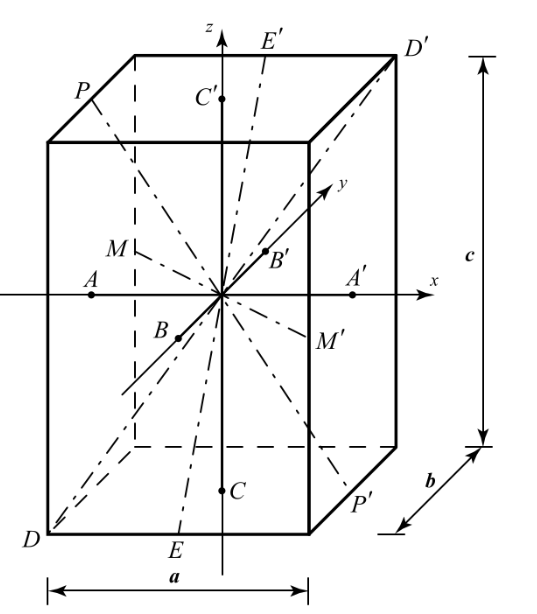
\includegraphics[scale=1]{kyb}
        \caption{Оси вращения прямоугольного параллелепипеда}
        \label{graphic1}
    \end{center}
\end{figure}

Момент инерции $I_{d}$ при вращении относительно диагонали DD' выражается
 через главные моменты с помощью формулы:
\begin{equation}
    I_{d}=I_{x}\frac{a^2}{d^2}+I_{y}\frac{b^2}{d^2}+I_{z}\frac{c^2}{d^2}
\end{equation}

Отсюда получаем соотношение
\begin{equation}
    (a^2+b^2+c^2)I^2_{d}=a^2 I_{x}+b^2 I_{y}+ c^2 I_{z}
\end{equation}
\quad\quadИспользуя связь момента инерции с периодом крутильных колебаний, получаем соотношение между периодами колебаний
\begin{equation}
    (a^2+b^2+c^2)T^2_{d}=a^2 T^2_{x}+b^2 T^2_{y}+c^2 T^2_{z}
\end{equation}
\quad\quad\ Соотношения между периодами колебаний относительно осей ЕE',
ММ' и PР' с периодами крутильных колебаний относительно главных осей
$$(b^2+c^2)T^2_{E}=b^2 T^2_{y}+c^2 T^2_{z}$$
$$(a^2+c^2)T^2_{P}=a^2 T^2_{x}+c^2 T^2_{z}$$
$$(a^2+b^2)T^2_{M}=a^2 T^2_{x}+b^2 T^2_{y}$$


\section{Методика измерений}

\begin{figure}[h]
                \centering
                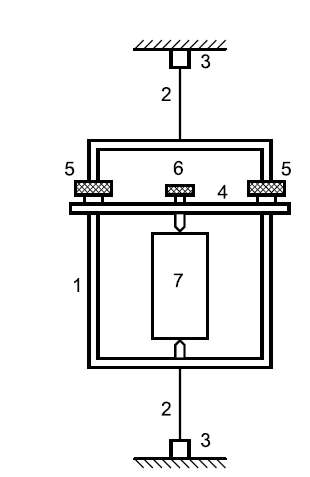
\includegraphics[width=0.3\linewidth]{ystanovka.png}
                \caption{Схема установки}
                \label{fig:mpr}
\end{figure}

\quad\quadВ данной работе используется устройство для получения крутильных колебаний, изображенное на риc. 2. Рамка 1 жестко соединена
с проволокой 2, закрепленной вертикально в специальных зажимах
3, позволяющих сообщить начальное закручивание для возбуждения
крутильных колебаний вокруг вертикальной оси. В рамке с помощью
планки 4, гаек 5 и винта 6 закрепляется твердое тело 7. На теле име-
ются специальные выемки, позволяющие его закрепить так, чтобы ось
вращения проходила в теле под различными углами через центр масс.

\section{Используемое оборудование}

\quad Установка для получения крутильных колебаний (жесткая рамка, имеющая винты для закрепления в ней твердых тел, подвешенная на натянутой вертикально проволоке), набор исследуемых твердых тел, секундомер.

\section{Результаты измерений и обработка данных}

\begin{itemize}
    \item Для начала установим геометрические параметры исследуемых тел. 
Штангенциркулем измеряем размеры и заносим в табличку. Для каждого тела по две таблицы: одна с измерениями, другая с получившимися средними значениями:

\begin{table}[!h]
    \centering
    \begin{tabular}{|l|l|l|} \hline
          & m, гр & a, см \\ \hline
        Куб & 1084.9 & 9.27  \\ \hline
    \end{tabular}
    \caption{Измерения для куба}
\end{table}
\begin{table}[!h]
    \centering
    \begin{tabular}{|l|l|l||l|l|l||l|l|l||l||l|} \hline
        a & 9.27 & 9.27 & 9.27 & 9.26 & 9.26 & 9.27 & 9.27 & 9.26 & 9.27 & 9.27 \\ \hline
        b & 9.26 & 9.27 & 9.27 & 9.26 & 9.27 & 9.26 & 9.26 & 9.27 & 9.26 & 9.27 \\ \hline
        c & 9.27 & 9.27 & 9.27 & 9.26 & 9.26 & 9.27 & 9.27 & 9.26 & 9.27 & 9.27 \\ \hline
    \end{tabular}
    \caption{Измерения сторон куба}
\end{table}

\begin{table}[!h]
    \centering
    \begin{tabular}{|l|l|l|l|} \hline
         & m, гр & d, см & h, см  \\ \hline
        Цилиндр & 2264 & 8.81 & 4.92  \\ \hline
    \end{tabular}
    \caption{Измерения для цилиндра}
\end{table}

\begin{table}[!h]
    \centering
    \begin{tabular}{|l|l|l||l|l|l||l|l|l||l||l|} \hline
        d & 8.82 & 8.81 & 8.81 & 8.81 & 8.82 & 8.81 & 8.81 & 8.81 & 8.82 & 8.81 \\ \hline
        h & 4.92 & 4.92 & 4.93 & 4.92 & 4.93 & 4.92 & 4.93 & 4.92 & 4.92 & 4.92 \\ \hline
    \end{tabular}
    \caption{Измерения сторон цилиндра}
\end{table}
\clearpage

\begin{table}[!ht]
    \centering
    \begin{tabular}{|l|l|l|l|} \hline
         & m, гр & d, см & h, см  \\ \hline
        Блин & 1569.5 & 12.44 & 1.68  \\ \hline
    \end{tabular}
    \caption{Измерения для блина}
\end{table}

\begin{table}[!ht]
    \centering
    \begin{tabular}{|l|l|l||l|l|l||l|l|l||l||l|} \hline
        d & 12.44 & 12.45 & 12.44 & 12.44 & 12.44 & 12.44 & 12.44 & 12.45 & 12.44 & 12.45 \\ \hline
        h & 1.68 & 1.68 & 1.68 & 1.69 & 1.69 & 1.68 & 1.68 & 1.69 & 1.68 & 1.69 \\ \hline
    \end{tabular}
    \caption{Измерения сторон блина}
\end{table}
\item Теперь по этим данным вычислим главные моменты инерции и их погрешность:
$$\varepsilon \approx \sqrt{\varepsilon^2_{a}+\varepsilon^2_{a}}\approx 0.1 \% $$
Поскольку $$\varepsilon^2_{a}\approx 0.1\%$$
\begin{description}
    \item[Куб]Для куба момент инерции относительно любой оси равны.
$$I_{z}= 9.32 \pm 0.01 \ \text{гр}\cdot \text{м}^2$$
    \item[Цилиндр]Моменты инерции относительно главных осей:
     $I_{z}$-относительно вертикальной оси, $I_{x}$-относительно горизонтальной оси.
$$I_{z}= 2.2 \pm 0.01 \ \text{гр}\cdot \text{м}^2, \ \ \ I_{x}= 2.65 \pm 0.01 \ \text{гр}\cdot \text{м}^2$$
\item[Блин]
$$I_{z}= 3.04 \pm 0.01 \ \text{гр}\cdot \text{м}^2, \ \ \ I_{x}= 3.07 \pm 0.01 \ \text{гр}\cdot \text{м}^2$$

\item[Цилиндр + блин]
$$I_{z}= 5.24 \pm 0.02 \ \text{гр}\cdot \text{м}^2, \ \ \ I_{x}= 5.72 \pm 0.02 \ \text{гр}\cdot \text{м}^2$$
\end{description}


    \item Далее определим периоды колебаний для пустой рамки, и всех остальных тел при различном положении
относительно оси колебаний. Отсчитваем 10-15 колебаний, проводя каждое измерение 3 раза.
Также перед каждой серией измерений убеждаемся в правильности выборе амплитуды: амплитуда выбрана правильно, если при уменьшении ее
в два раза период колебаний, определяемый по 10-15 колебаниям, остается тем же. Заносим данные для разных фигур в табличку.
Погрешность измерения времени обусловлена ошибкой округления и равна: $\varepsilon_{T} \approx 0.5 \% $ при 10 измерениях и $\varepsilon_{T} \approx 0.3 \% $ при 15 измерениях.

\begin{description}
    \item[Рамка]Измерения для рамки: 
    \begin{table}[!ht]
        \centering
        \begin{tabular}{|l|l|l|l|l|l||l|l|} \hline
            Рамка & $N$ & $t_{N1}$,с & $t_{N2}$,с & $t_{N3}$,c & $t_{N4}$,c & $t_{N5}$,c & $T$,c \\ \hline
            $T_{OZ}$ & 10 & 44.82 & 44.71 & 44.7 & 44.4 & 44.65 & 4.47 \\ \hline
        \end{tabular}
    \end{table}
    \item[Цилиндр]Измерения для цилиндра:
    \begin{table}[!ht]
        \centering
        \begin{tabular}{|l|l|l|l|l|l|l||l|l|}
        \hline
            Цилиндр & $N$ & $t_{N1}$,с & $t_{N2}$,с & $t_{N3}$,c & $T$,c &
            $1/\sqrt{T^2-T^2_{p}}, 10^{-2} c^{-1}$  \\ \hline
            $T_{OZ}$ & 10 & 56 & 56.2 & 56.2 & 5.61 & 29.5  \\ \hline
            $T_{OX}$ & 10 & 53 & 53.2 & 53.3 & 5.32 & 34.67  \\ \hline
        \end{tabular}
    \end{table}

    \item[Куб]Измерения для куба:
    \begin{table}[!ht]
        \centering
        \begin{tabular}{|l|l|l|l|l|l|l|}
        \hline
            куб & $N$ & $t_{N1}$,с & $t_{N2}$,с & $t_{N3}$,c & $T$,c & $1/\sqrt{T^2-T^2_{p}}, 10^{-2} c^{-1}$  \\ \hline
            $T_{EE'}$ & 10 & 53.9 & 54 & 54.1 & 5.4 & 33.01  \\ \hline
            $T_{DD'}$ & 10 & 53.6 & 53.2 & 53.3 & 5.34 & 34.23  \\ \hline
            $T_{OZ(CC')}$ & 10 & 53.6 & 53.63 & 53.5 & 5.36 & 33.81  \\ \hline
        \end{tabular}
    \end{table}
    \clearpage
    \item[Блин]Измерения для блина:
    \begin{table}[!ht]
        \centering
        \begin{tabular}{|l|l|l|l|l|l|l||l|l|}
        \hline
            Блин & $N$ & $t_{N1}$,с & $t_{N2}$,с & $t_{N3}$,c & $T$,c &
            $1/\sqrt{T^2-T^2_{p}}, 10^{-2} c^{-1}$  \\ \hline
            $T_{OZ}$ & 10 & 53.68 & 53.86 & 54.16 & 5.39 & 33.2  \\ \hline
            $T_{OX}$ & 10 & 53.19 & 53.34 & 53.15 & 5.32 & 34.67  \\ \hline
        \end{tabular}
    \end{table}
    \item[Цилиндр + блин]Измерения для цилиндра и блина:
    \begin{table}[!ht]
        \centering
        \begin{tabular}{|l|l|l|l|l|l|l||l|l|}
        \hline
            Цилиндр + блин & $N$ & $t_{N1}$,с & $t_{N2}$,с & $t_{N3}$,c & $T$,c &
            $1/\sqrt{T^2-T^2_{p}}, 10^{-2} c^{-1}$  \\ \hline
            $T_{OZ}$ & 10 & 71.5 & 71.2 & 70.9 & 7.12 & 18.04  \\ \hline
        \end{tabular}
    \end{table}
\end{description}

\item Теперь по полученным ранее данным построим эллипсоид инерции для параллелограмма и куба. За длину радиус вектора примим
$r=100/\sqrt{T^2-T^2_{p}}$. Строить эллипсы будем методом наименьших квадратов. Т.к параметричеческое ур-ие эллипса выглядит как:\\
$y=b \cdot \sin(\varphi), x= a \cdot \cos(\varphi)$ То зависимость координаты $x,y$ от соответственно $sin(\varphi),\cos(\varphi)$ линейная и
проходит через начало координат. Тогда зная 
длину радиус вектора и углы под которыми направлены побочные оси к главным осям, проводим аппроксимацию методом наименьших квадратов
 и строим эллипс с полученными параметрами.
$$a=\frac{\langle x \cdot \cos(\varphi)\rangle }{\langle \cos(\varphi)^2 \rangle }, \ \ \ b=\frac{\langle y \cdot \sin(\varphi)\rangle }{\langle \sin(\varphi)^2 \rangle }$$
\begin{description}
    \item[Цилиндры]Блин: $a = 34.67 \cdot 10^{-2}c^{-1}$ ,$b = 33.2 \cdot 10^{-2}c^{-1}$\\
Цилиндр: $a = 34.67  \cdot 10^{-2}c^{-1}$ ,$b = 29.5 \cdot 10^{-2}c^{-1}$
    \item[Куб] Для куба эллипсоид инерции - шар. Примем за его радиус средний по
всем сериям измерений. $r = 33.68 \cdot 10^{-2}c^{-1}$
\end{description}
\item Проверим насколько теоретически предсказанные моменты инерции для цилиндров относительно
главных осей с полученным экспериментальным результатоом, пользуясь тензором инерции.
Вычислим отношения моментов инерции вдоль главных осей. Погрешность экспериментального значения оценим как:\\
$\varepsilon_{Ji/Jj}=2\sqrt{\varepsilon^2_{ri}+\varepsilon^2_{rj}} \approx 10 \%$\\
Погрешность теоретического пренебрежимо мала и порядка $1\%$.\\
Теоретическое значение для цилиндра: $I_{x}/I_{z}= 1.4$, экспреиментальное $I_{x}/I_{z}=c^2/a^2=1.38 \pm 0.1$\\
Теоретическое значение для блина: $I_{x}/I_{z}= 1$, экспреиментальное $I_{x}/I_{z}=c^2/a^2=1.08 \pm 0.1$\\

\end{itemize}

\newpage
\begin{figure}[h]
                \centering
                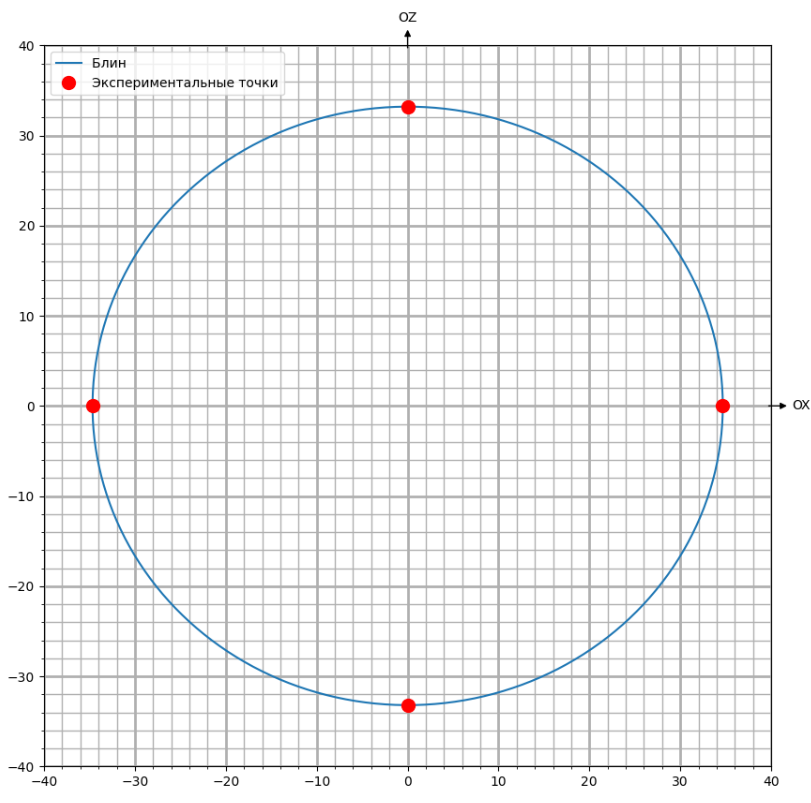
\includegraphics[width=0.7\linewidth]{blin.png}
                \caption{Эпсилоид инерции для блина}
                \label{fig:mpr}
\end{figure}

\begin{figure}[h]
                \centering
                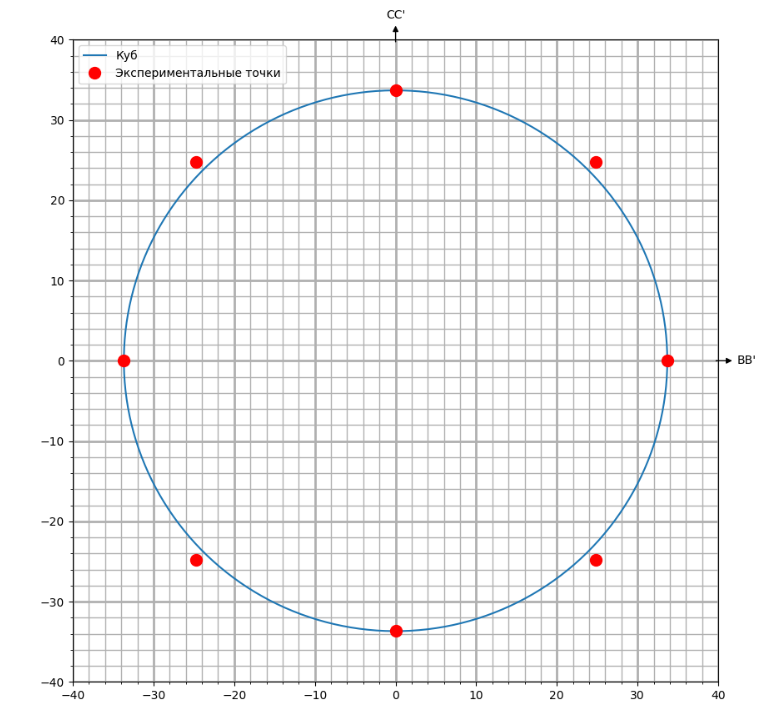
\includegraphics[width=0.7\linewidth]{kub.png}
                \caption{Эпсилоид инерции для куба}
                \label{fig:mpr}
\end{figure}
\clearpage

\begin{figure}[h]
                \centering
                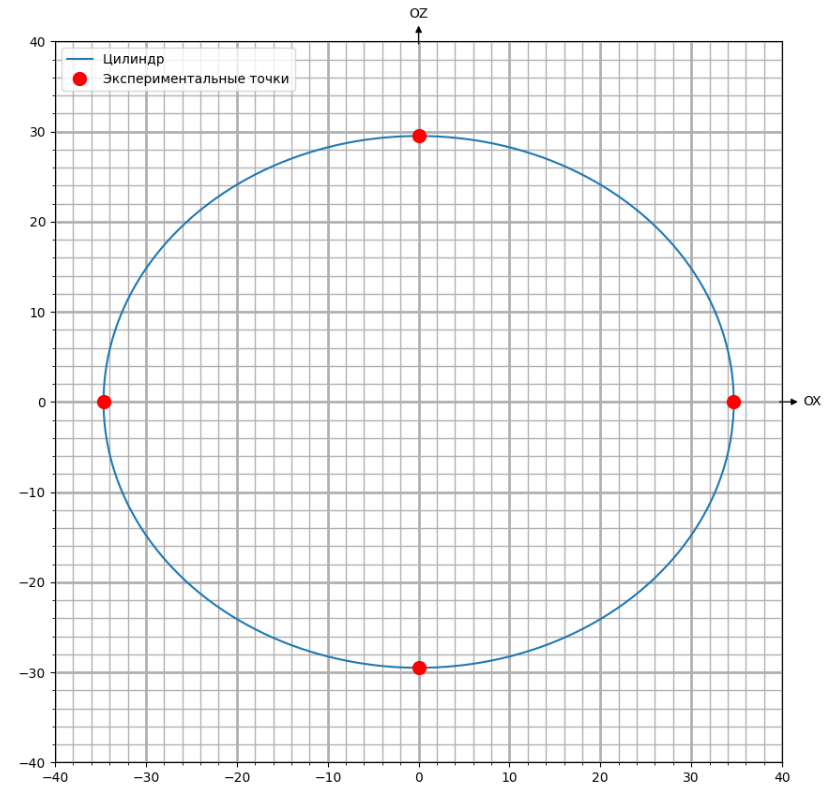
\includegraphics[width=0.7\linewidth]{tsilindr.png}
                \caption{Эпсилоид инерции для цилиндра}
                \label{fig:mpr}
\end{figure}
\section{Обсуждение результатов}
Можем заметить, что точки не идеально ложатся на построенную кривую, что вероятно обсуловленно
особенностями установки(затуханием,провисанием или возникающими эффектами) и случайной погрешностью, связанной
со скоростью реакции человека. Таким образом использование нашей установки дает некоторую приличную погрешность, 
но ее точности вполне достаточно для получения интересующих нас выводов. Поэтому, так как точки хорошо ложатся на эллипс,
мы можем сделать вывод о справедливости теоретических формул.
\section{Вывод}В ходе работы были измерены периоды колебаний относительно различных осей.
Была подтверждена теоретическая зависимость между периодами крутильных колебаний тела относительно 
различных осей. По ним были установлены положения главных осей тела и вычислены моменты инерции относительно этих осей.
По этим данным был построен вид эллипсоида инерции.
По виду эллипсоида инерции были вычислены соотношения между моментами инерции тела относительно главных осей,
которые совпадают с теоретическим расчетом в пределах погрешности.

\end{document}